\section{Measurement}\label{sec:measurement}
This section will describe the previous CLAS preliminary result on the \etaTP \ analysis performed with the g12 experiment. Also in this section is a description on how the \etaDal \ and \ \phiDal \ were simulated and reconstructed for this CLAS12 proposal.
\subsection{Previous CLAS analyses}
The g12 experiment performed at CLAS produced data set of photon-induced reactions. Fortunately, the Cherenkov Counters(CC) were filled with perflourbutane ($C_4F_{10}$) and a trigger consisting of a coincidence between the (ST$\cdot$TOF)(CC$\cdot$EC) allowing the study of dilepton reactions throughout the entire beam energy range $1.15 \ \mathrm{GeV}<E_\gamma <5.45 \ \mathrm{GeV}$. Preliminary analyses of g12 involving dileptons include the decays:
\begin{itemize}
\item $\Delta \to p \epem$ (Transition form factor)
\item $\eta \to \epem \gamma$ (Transition form factor)
\end{itemize}

while advanced analyses involving dileptons include:
\begin{itemize}
\item $\piz \to \epem \gamma$ (Differential Cross-Section)
\item $\omega / \rho \to \epem$ (Interference of $\omega/\rho$ )
\item $\omega \to \epem \piz$ (Transition form factor)
\item $\etaP \to \epem \gamma$ (Transition form factor / branching ratio)
\end{itemize}
\missingfigure{g12plots}
As seen in Fig. the current CLAS results suffer from insufficient statistics. Therefore, we propose to repeat the \etaPDal \  measurement with CLAS12.
\subsection{Simulating and Reconstruction}
To simulate the reactions in Eq.~\ref{eq:etaP} and Eq.~\ref{eq:phiP}, the program PLUTO++~\cite{PLUTO} was utilize for its ability to simulate the decays of those according to QED, Vector Meson Dominance or a user inputted TFF. For reconstruction of the desired topologies, the CLAS12 FASTMC was used, in which $\sim 9\cdot10^6$ events were generated for \etaPDal \ and \phiDal \ and then simulated with FASTMC at 75\% torus field. An extra simulation was performed for the torus field setting of 100\% to show the effects of the magnetic field on the lepton acceptance. All detector efficiencies are assumed to be 100\% except the EC efficiency, in which an efficiency of 10\% was factored for each detected lepton. This EC efficiency was calculated with the g12 data set and the assumption is that the CLAS12 EC efficiency will be at least the same as the previous CLAS EC since the EC is the same sub-detector in both detectors.

\indent The production of each particle was weighted by photo-production 
differential cross-sections, $\frac{d\sigma}{d\Omega}(v,\cos\theta_{cm})$, published in~\cite{Williams}, where $v$ is the virtual photon energy. This was done to achieve a quasi realistic model of the production. The \epemT \  decay spectrum, of each meson, was weighted via the VMD model (including QED predictions). Another simulation was performed using a flat $M(\epem)$ distribution (No QED, No VMD) to analyze any effects of the model on the \epemT acceptance. The analysis showed that this acceptance was independent of the decay model, see Fig.\ref{fig:VMDaccepted} and Fig.\ref{fig:FLATaccepted}.
\subsubsection{Reconstruction And Acceptance}\label{sec.reconstruction}
An exclusive reconstruction scheme
\begin{align}
ep\to e'p \etaP \rightarrow p e^+e^- \gamma  \\
ep\to e'p \phi \rightarrow p e^+e^- \eta \ ,
\end{align}
where all final state particle are detected, as well as an inclusive reconstruction scheme
\begin{align}
ep\to e'p \etaP \rightarrow e^+e^- \gamma (p) \\
\end{align}
where the proton was not detected, was analyzed. Figure~\ref{fig:VMD} and Fig.~\ref{fig:FLAT} show the generated \epemT \ spectrum along with the accepted events for both reconstruction schemes. The acceptance was calculated by dividing the accepted events by the generated events, per $M(\epem)$ bin. The $\etaP$ Dalitz decay acceptance can be seen in Fig.\ref{fig:VMDaccepted} and the $\phi$ Dalitz decay acceptance in Fig.\todo{add reference to plot once done}.
\begin{figure}[h!]\begin{center}
		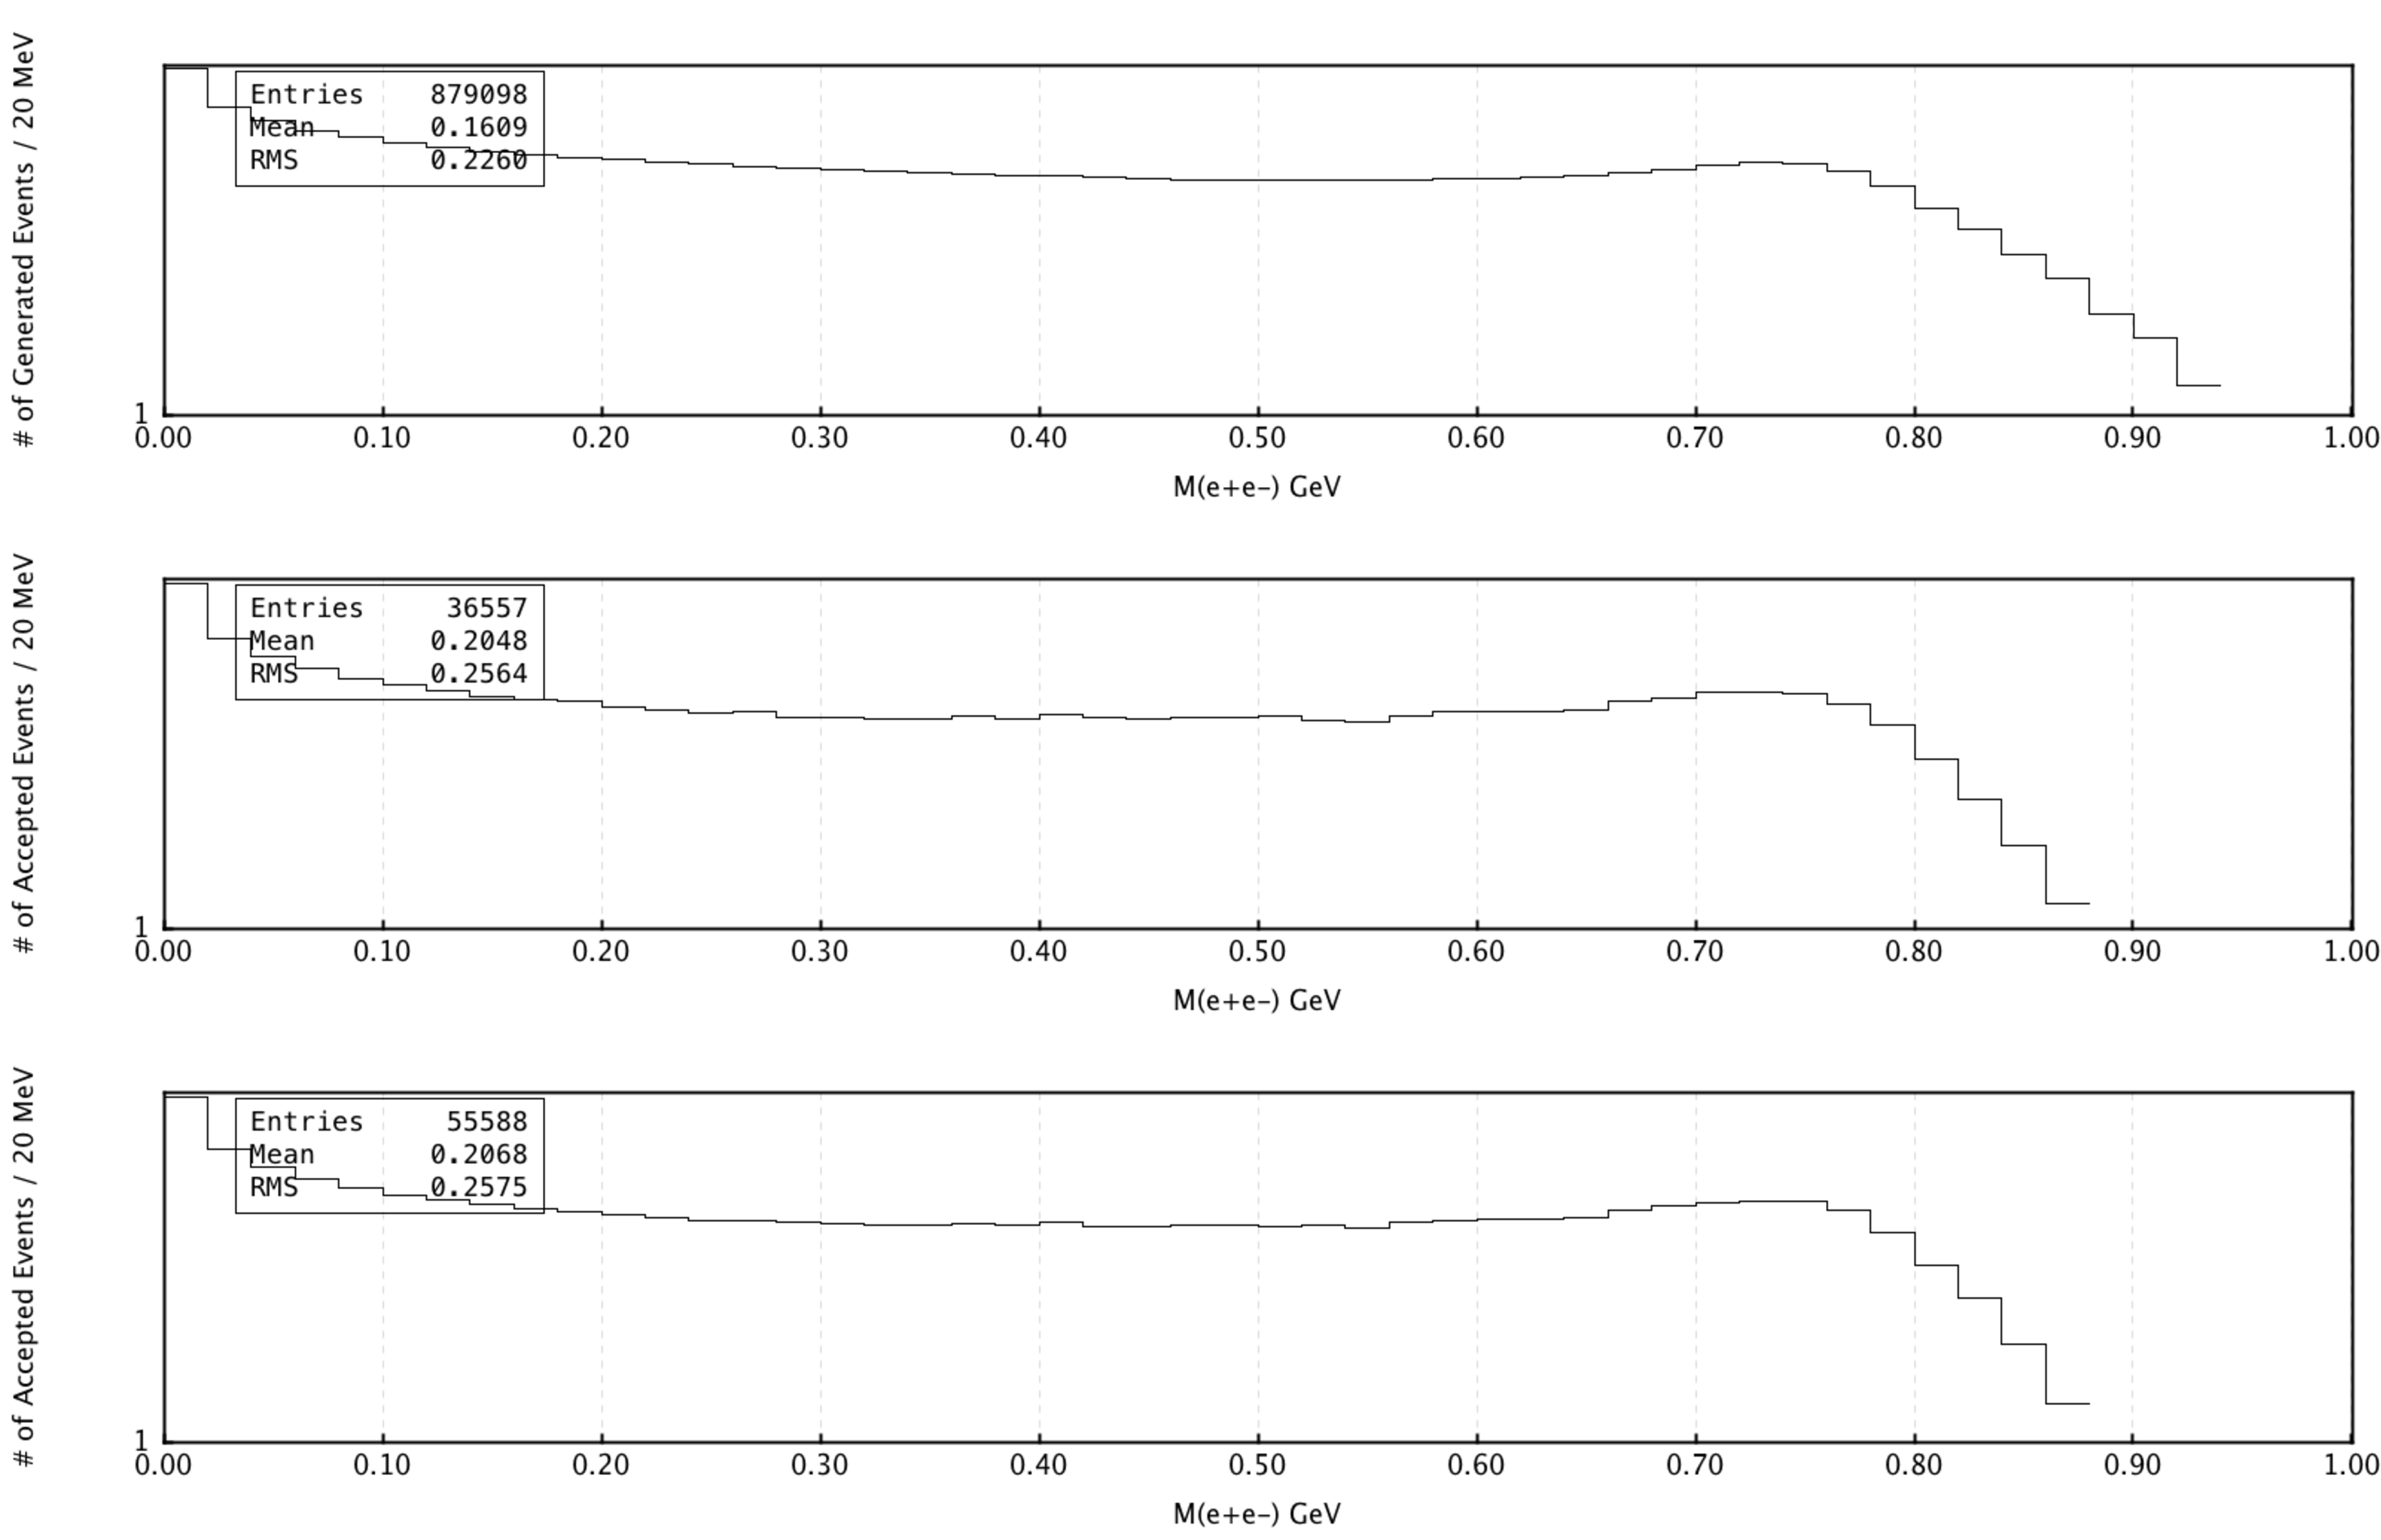
\includegraphics[width=\figwidth,height=2.6\qfigheight]{\grpath/counts/75_TORUS/VMD/VMD_Generated_Accepted.pdf}
		\caption[Generated and Accepted counts, as a function of $M(\epem)$]{\label{fig:VMD}{Generated events (Top), accepted events for an exclusive (Middle), inclusive(Bottom) reconstruction schemes as a function of $M(\epem)$. In all panels a VMD decay model was employed}}
\end{center}\end{figure}
\begin{figure}[h!]\begin{center}
			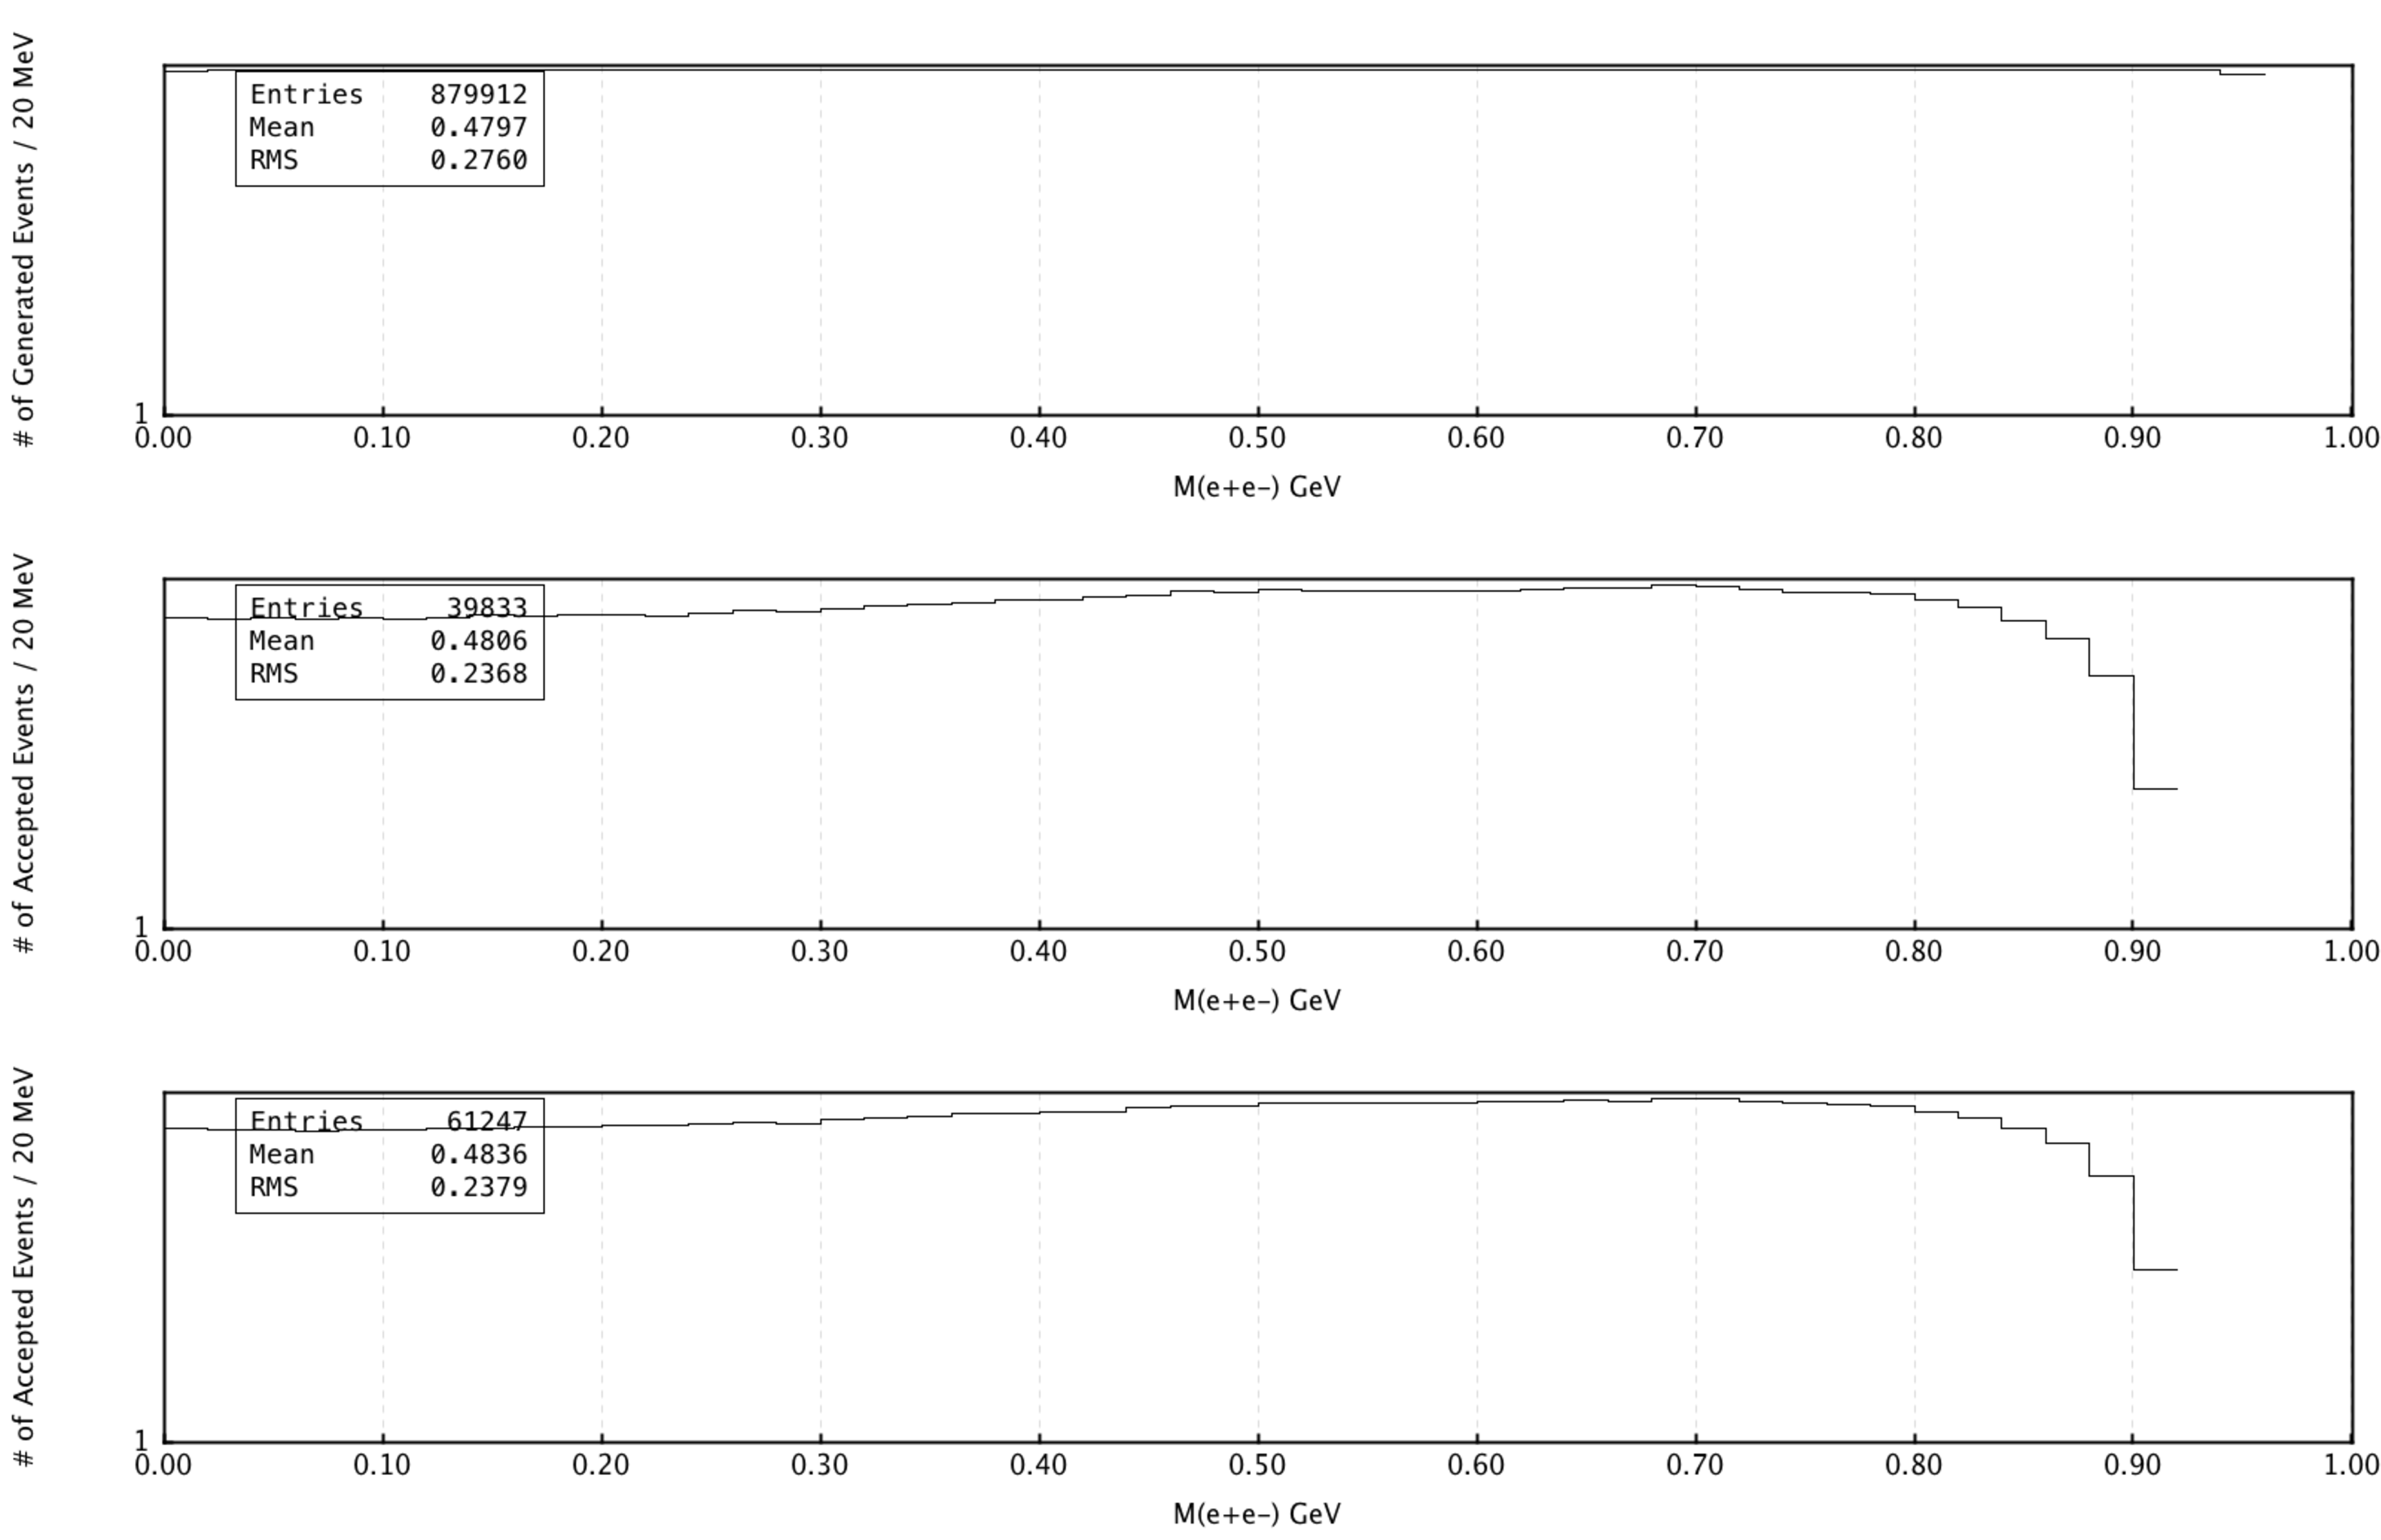
\includegraphics[width=\figwidth,height=2.6\qfigheight]{\grpath/counts/75_TORUS/FLAT/FLAT_Generated_Accepted.pdf}
			\caption[Generated and Accepted counts, as a function of $M(\epem)$]{\label{fig:FLAT}{Generated events (Top), accepted events for an exclusive (Middle), inclusive(Bottom) reconstruction schemes as a function of $M(\epem)$. In all panels a Flat \epemT \ decay model was employed}}
\end{center}\end{figure}
\FloatBarrier

\begin{figure}[h!]\begin{center}
		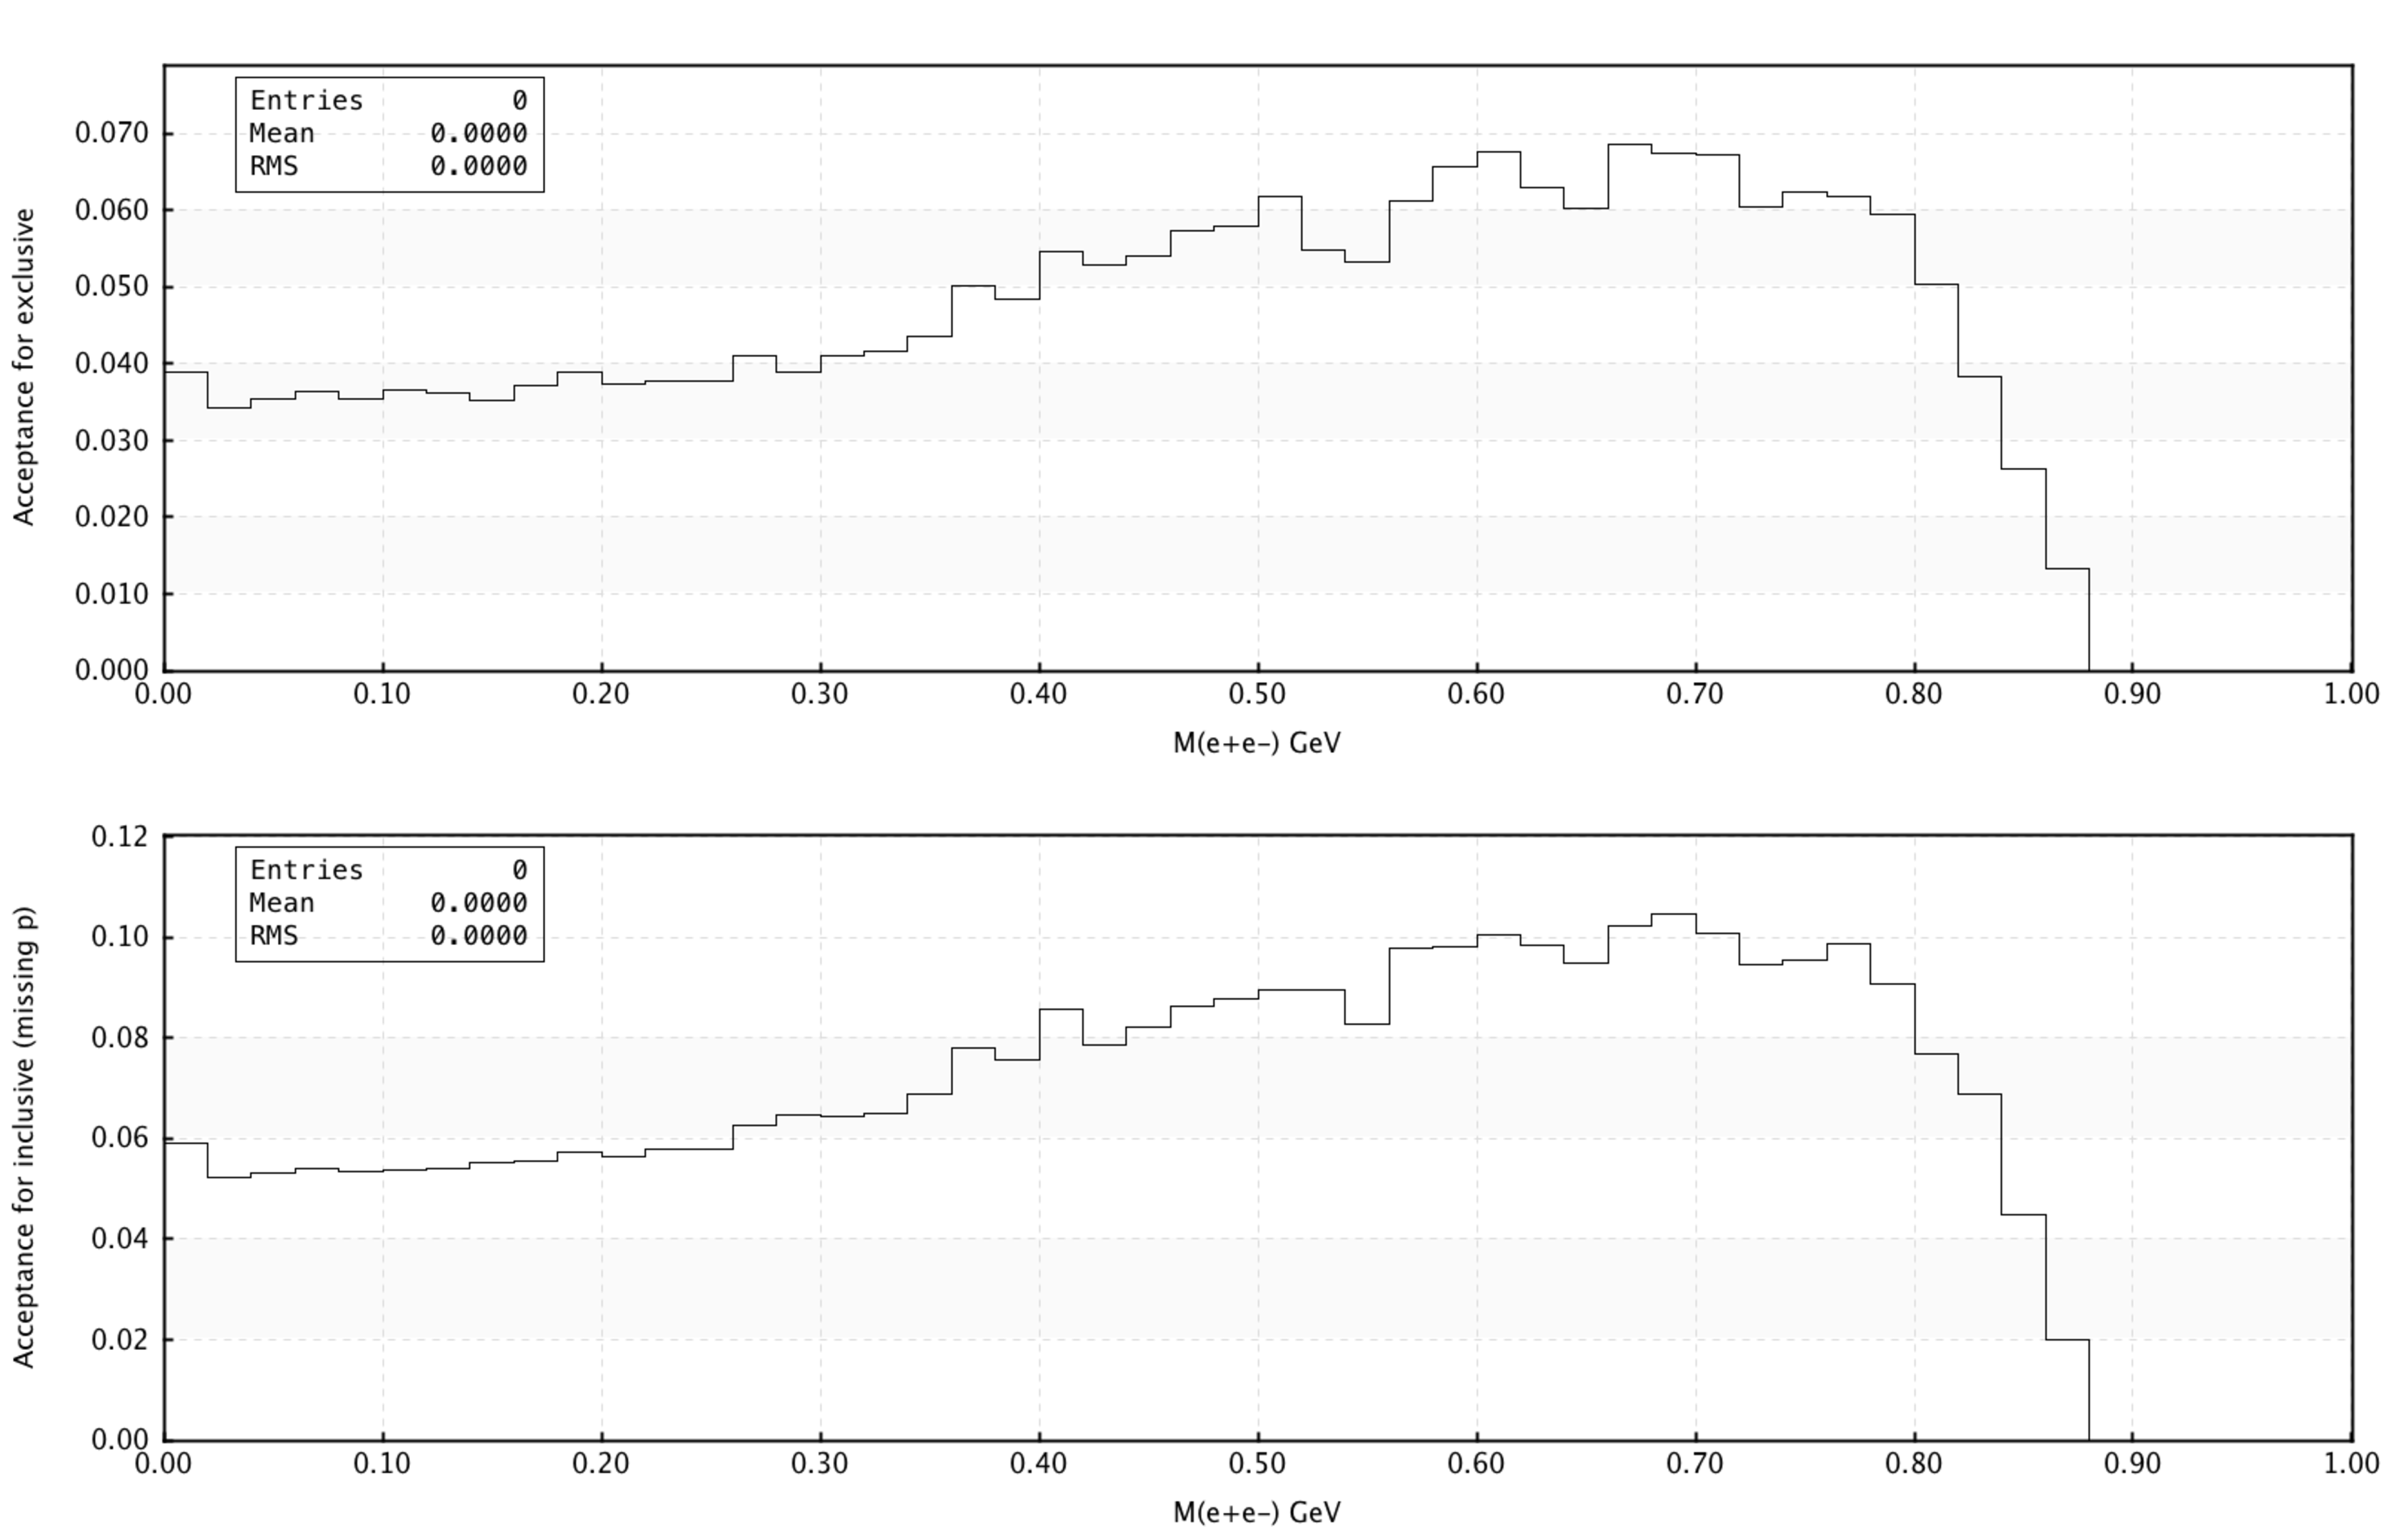
\includegraphics[width=\figwidth,height=1.2\qfigheight]{\grpath/counts/75_TORUS/VMD/VMD_Acceptance.pdf}
		\caption[Acceptance, as a function of $M(\epem)$]{\label{fig:VMDaccepted}{Acceptance using a VMD decay model, as a function of $M(\epem)$ for the exclusive (Top) and inclusive reconstruction scheme(Bottom). }}
\end{center}\end{figure}

 \begin{figure}[h!]\begin{center}
 		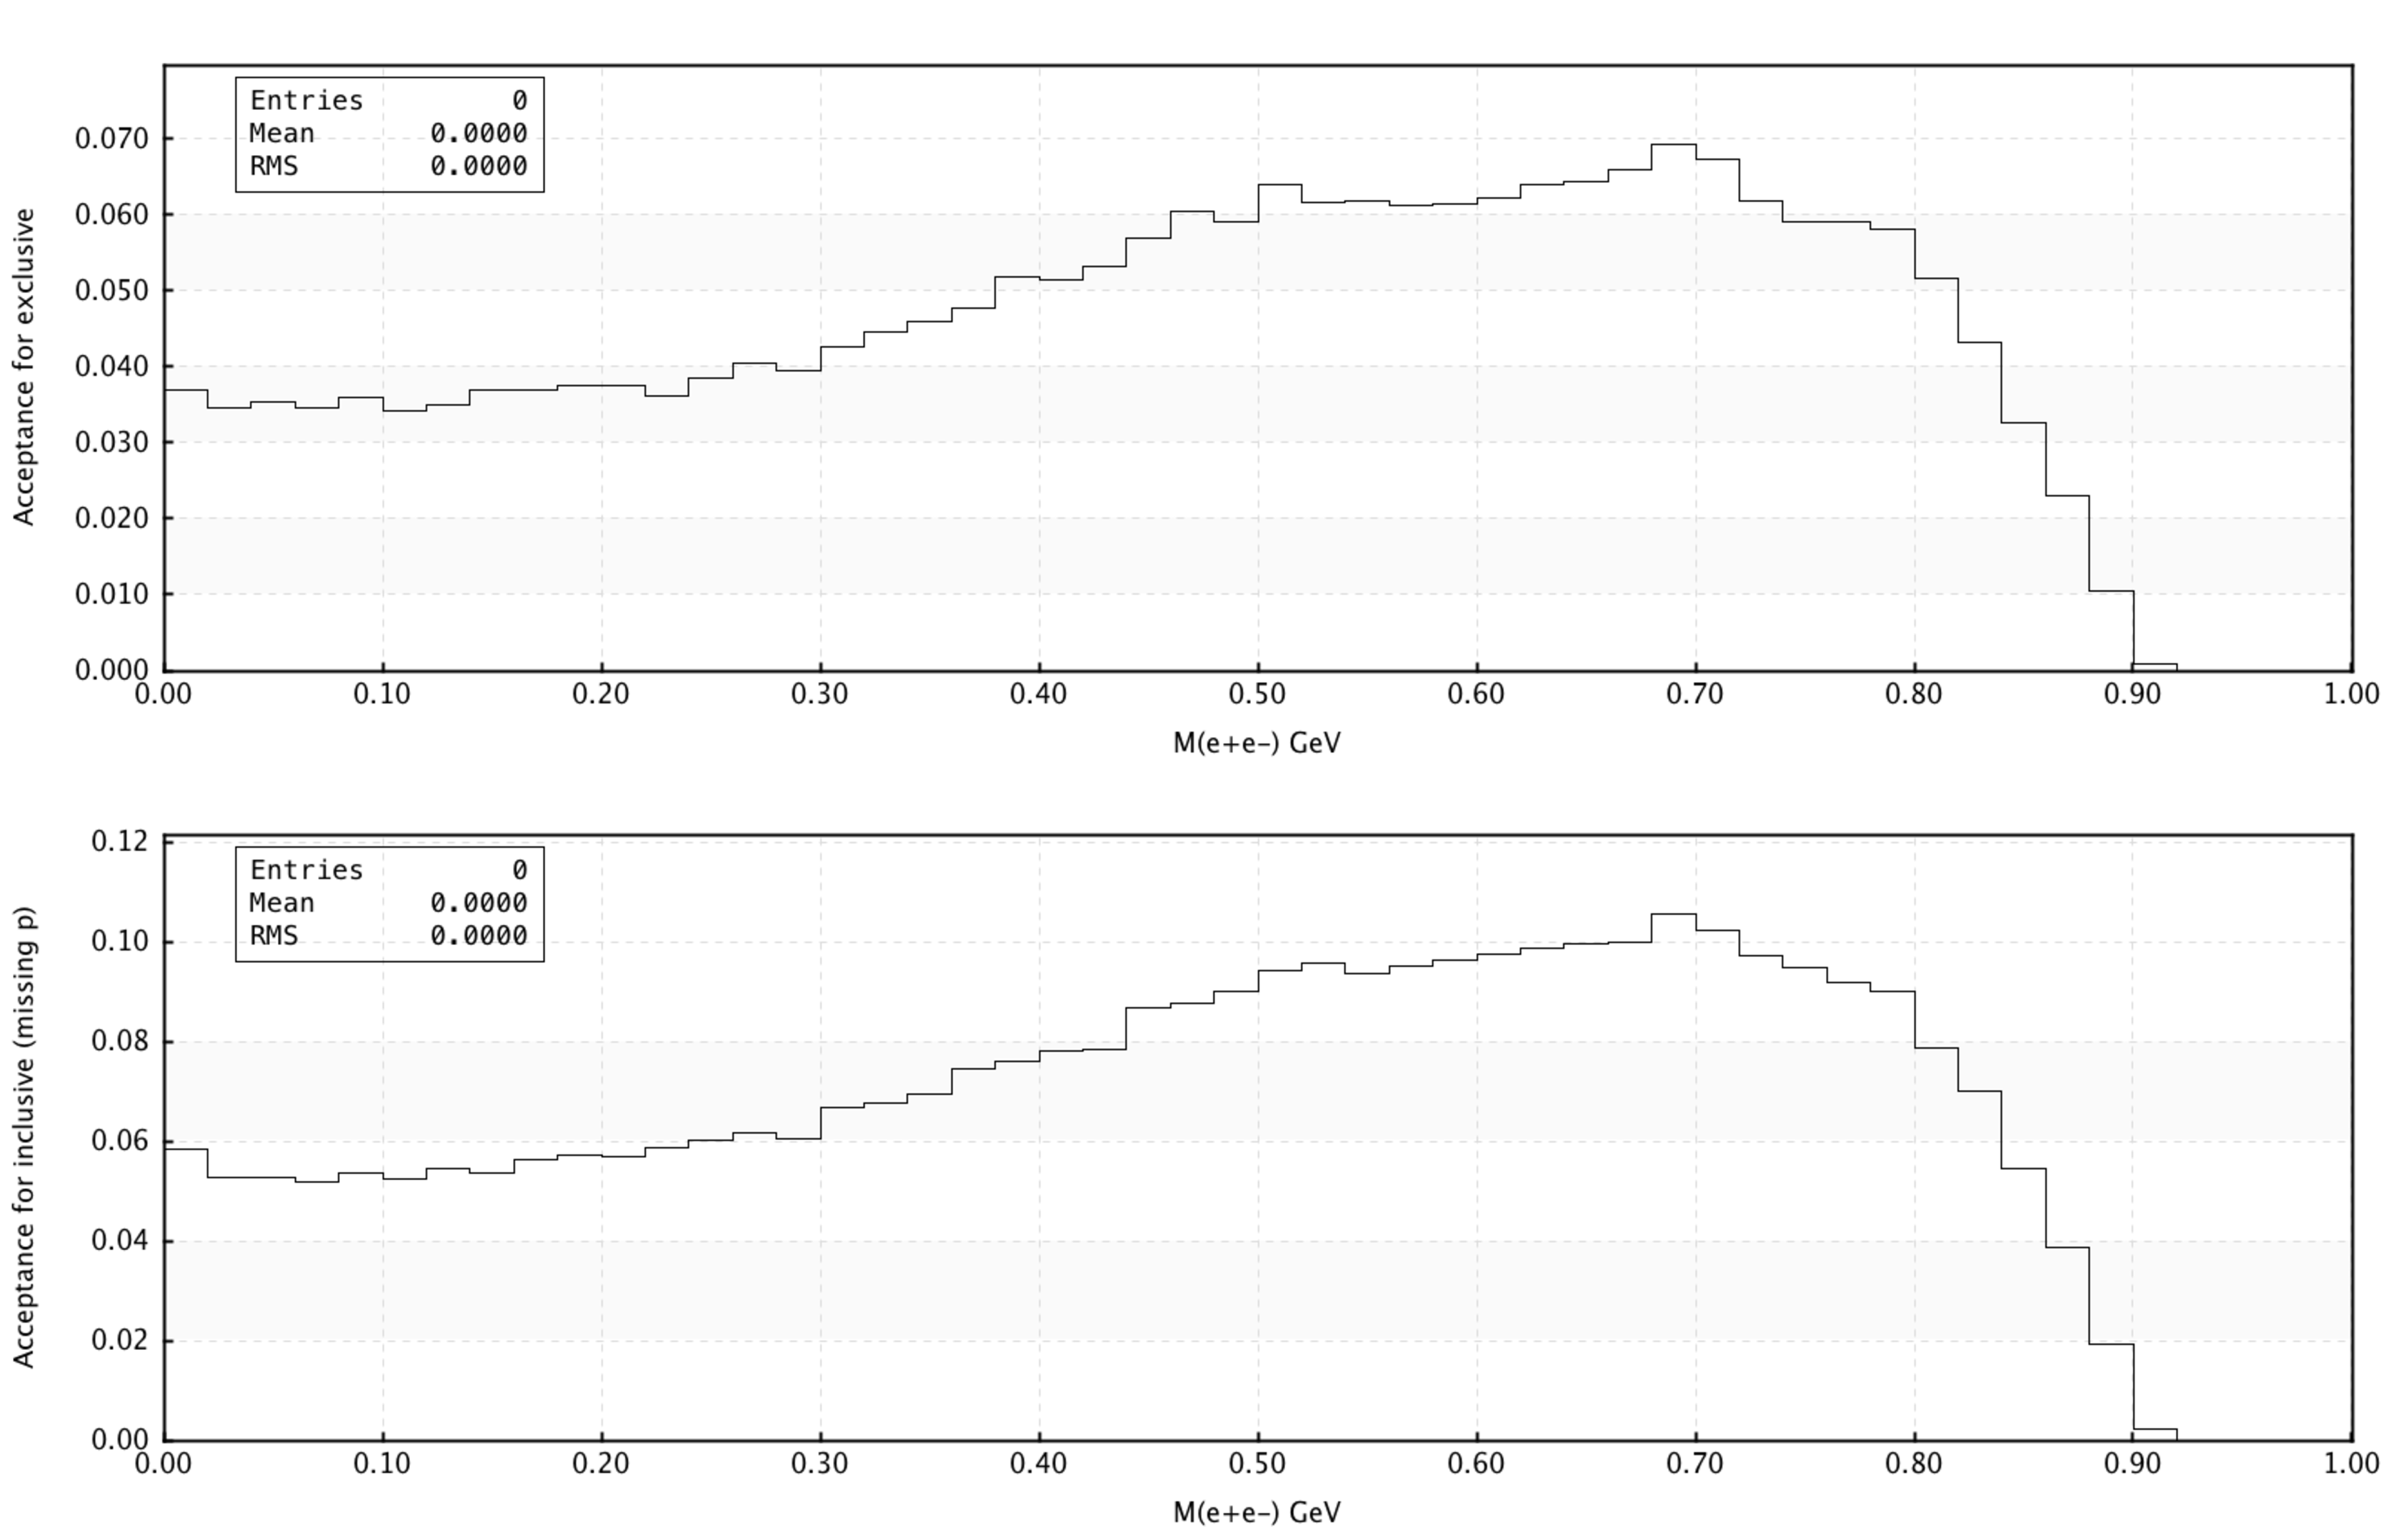
\includegraphics[width=\figwidth,height=1.2\qfigheight]{\grpath/counts/75_TORUS/FLAT/FLAT_Acceptance.pdf}
 		\caption[Acceptance, as a function of $M(\epem)$]{\label{fig:FLATaccepted}{Acceptance using a flat \epemT \ decay model, as a function of $M(\epem)$ for the exclusive (Top) and inclusive reconstruction scheme(Bottom).}}
 \end{center}\end{figure} 
\FloatBarrier
\subsection{Calculating Expected Yield}
\subsubsection{Calculating Photon Flux}\label{sec:calflux}
A simple method for calculating the photon flux in CLAS12 is as follows; Using the fact that g12 had a photon flux of $7\cdot 10^7 \ \mathrm{\gamma/s}$ on a Au radiator of $10^{-4} \chi_0$ an expected $\sim 4\cdot 10^9  \mathrm{\gamma/s}$ will be seen in CLAS12 at ${\cal L} = 10^{35}\mathrm{cm^{-2}s^{-1}}$ on a 5~cm $\ell H_2$ target which is $\sim 5.7\cdot 10^{-3} \chi_0$. This number has been independently confirmed in a previous CLAS proposal~\cite{clas.proposal.meson}.
\subsubsection{Calculating Yield}
The average number of $\mathrm{meson} \to \epem X$ expected in CLAS12 can be calculated as:
\begin{align}
\bar{N}(\epem)_{\mathrm{meson}  \to \epem X} = \Phi \epsilon(\epem)\bar{\sigma} \rho_{\ell_{H_2}}\ell_{target}N_A \frac{\Gamma_{\mathrm{tot}_\mathrm{meson} }}{\Gamma_{\mathrm{meson}  \to \epem X}}\ ,
\end{align}
where $\Phi$ is the photon flux estimated in Sec.~\ref{sec:calflux}, $\epsilon$ is the acceptance, $\bar{\sigma}$ is the total cross-section, $\rho_{\ell_{H_2}}$ is the atomic density of $\ell_{H_2}$, $\ell_{target}$ is the target length, $N_A$ is Avogadro's constant, and $\frac{\Gamma_{\mathrm{tot}_\mathrm{meson}}}{\Gamma_{\mathrm{meson} \to \epem X}}$ is the total branching fraction of the meson decaying into $\epem X$.
Using the lepton acceptance shown is Sec.~\ref{sec.reconstruction} the average number of \etaTP \  per $M(\epem)$ can be seen in Fig.~\ref{fig:etayield}.
 \begin{figure}[h!]\begin{center}
 \subfloat[$\etaP$ Dalitz and conversion spectra][]{ %Feynman diagram of $\etaP$ two photon decay
	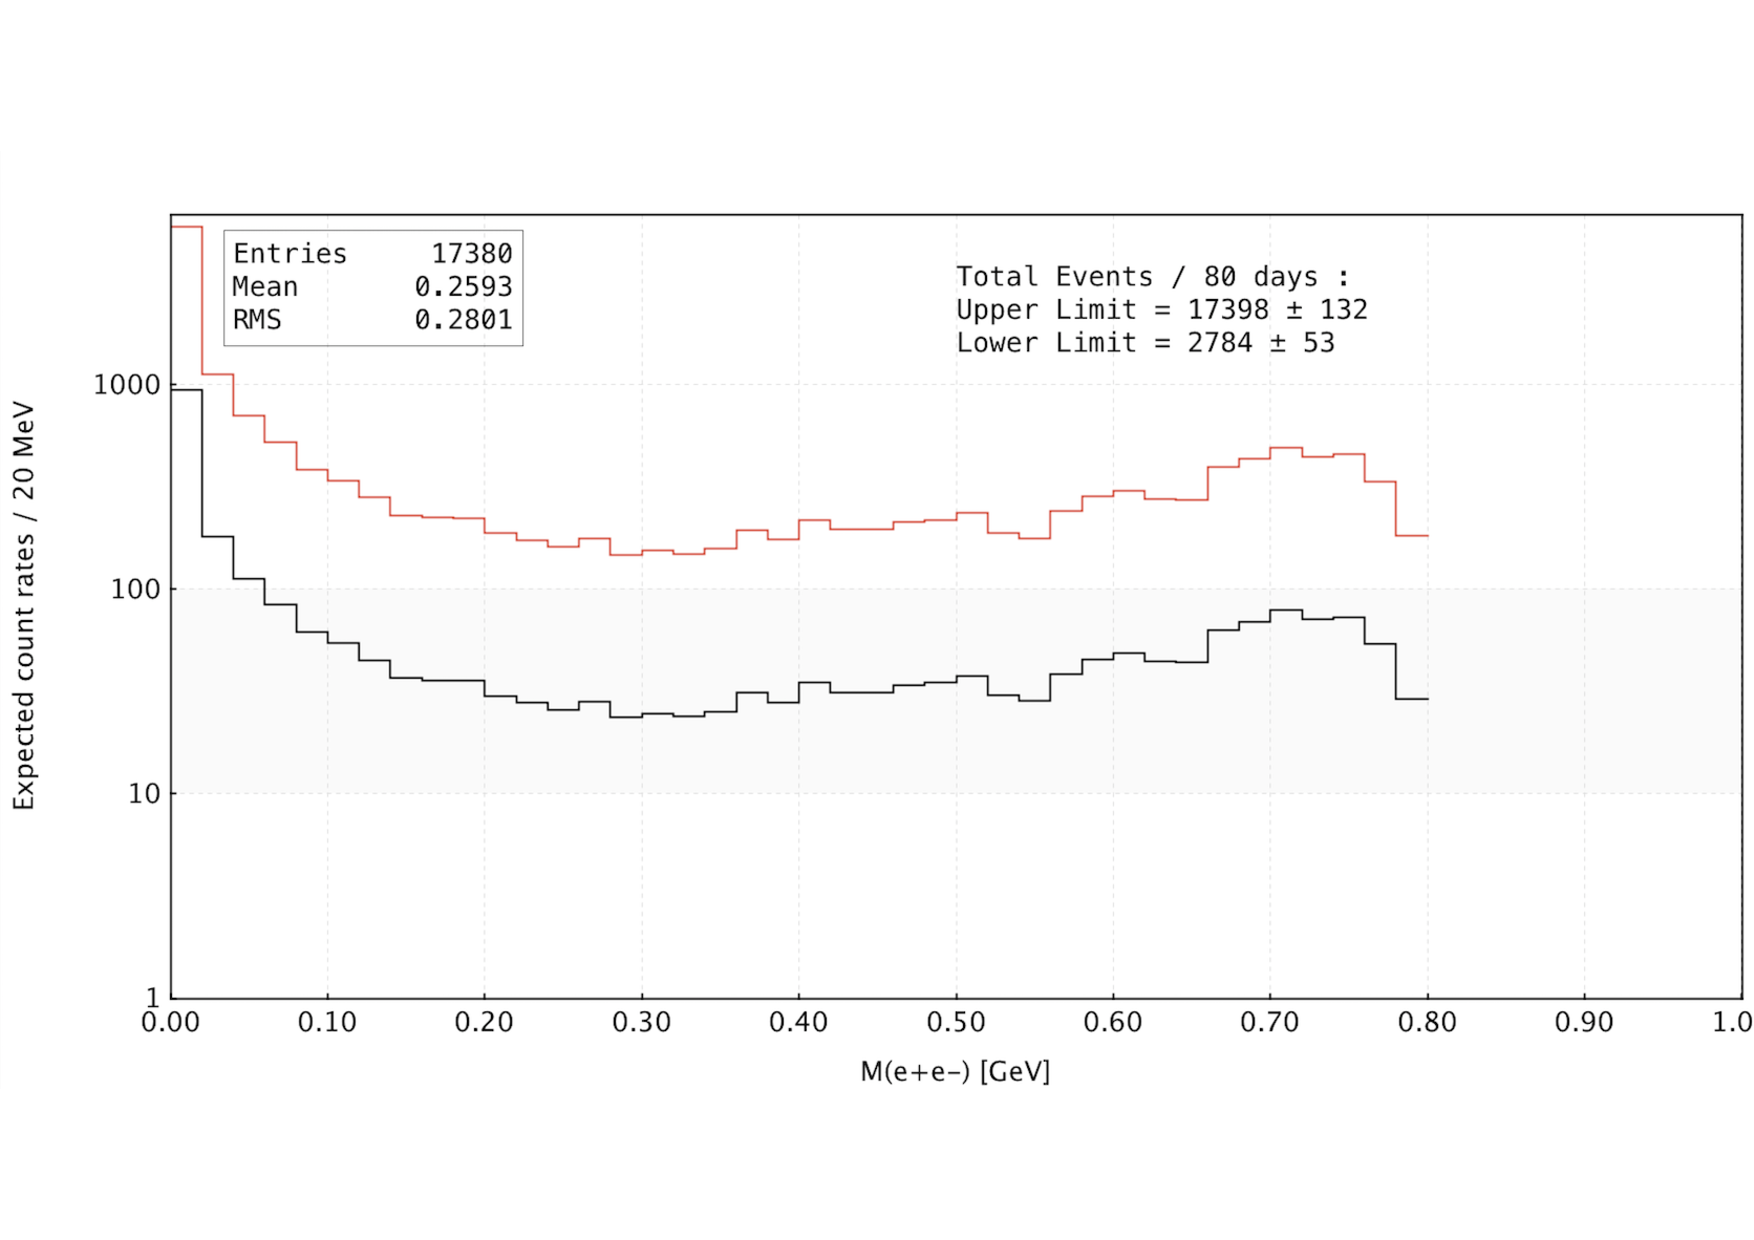
\includegraphics[width=0.8\columnwidth,height=1.0\qfigheight]{\grpath/counts/75_TORUS/VMD/VMD_Excluvise_count_rate.pdf}\label{fig:etap_count_exclu}
	}
\\
\subfloat[$\phi$ Dalitz and conversion spectra][]{ %Feynman diagram of $\etaP$ Dalitz decay
	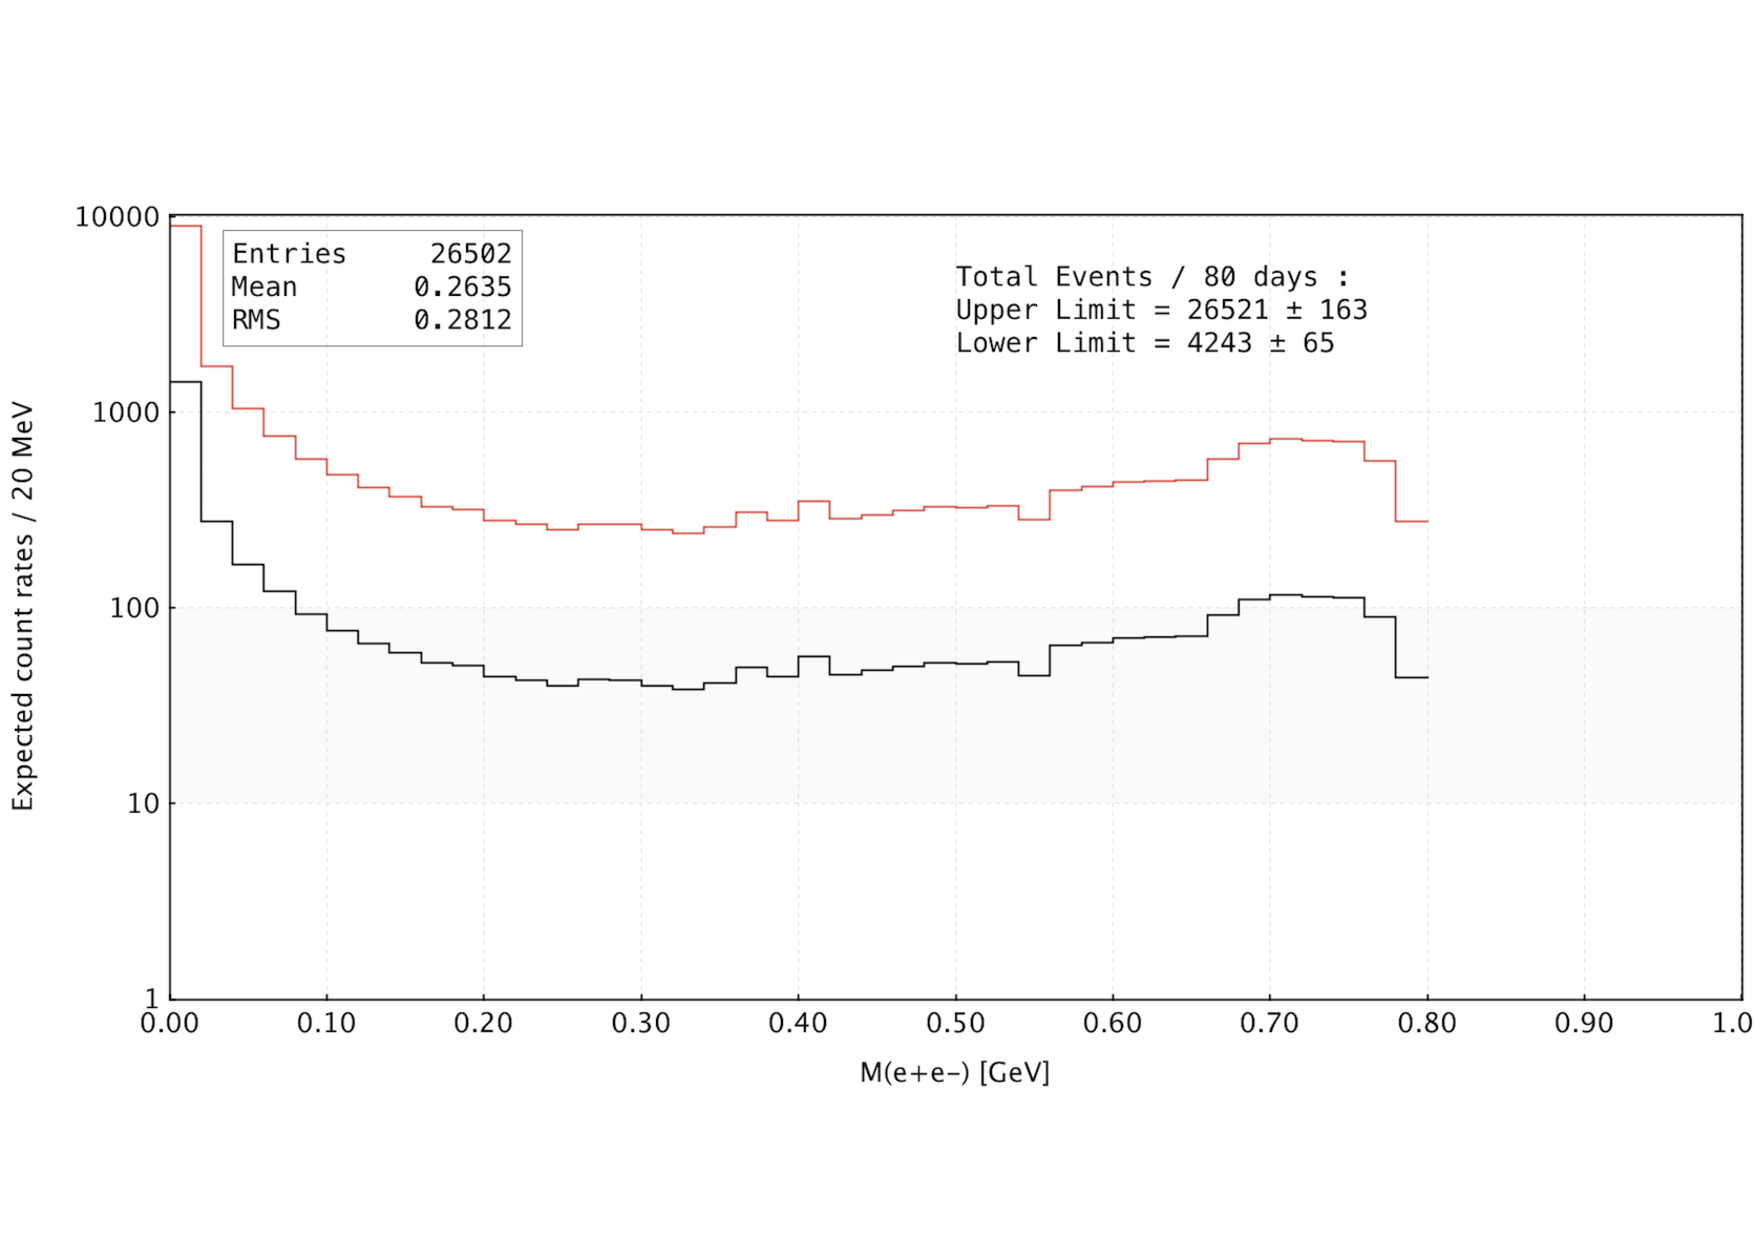
\includegraphics[width=0.8\columnwidth,height=1.0\qfigheight]{\grpath/counts/75_TORUS/VMD/VMD_Incluvise_count_rate.pdf}\label{fig:etap_count_inclu}
	}
\caption[Counts rates for \etaTP]{\label{fig:etayield}Count rates for the exclusive~\subref{fig:etap_count_exclu} and inclusive~\subref{fig:etap_count_inclu}. For both plots the photon detection efficiency was assumed to be between 10\%(Red) and  2\%(Black). }
\end{center}\end{figure}
\FloatBarrier
Integrating over $M(\epem)$, the expected yield calculates to be $17,398$ events for exclusive scheme and $26,521$ events for the inclusive scheme. This would increase the world statistics by a factor of $\sim 20$ and $\sim 30$ respectively. 
Table~\ref{tab:counts} and Tab.~\ref{tab:countsfull} in App.~\ref{sec:app.rates} depicts the upper and lower amount of \epemT expected from 80 days of beam time for two torus fields of 75\% and 100\% respectively.
\FloatBarrier
\subsection{Realistic Yield}
As a reality check, lets compute the number of $\etaP \to \epem \gamma$ that g12 would have seen, had the experiment ran for 80 days with a real photon flux as calculated for CLAS12 (Sec.~\ref{sec:calflux}). %with the \epemT trigger configuration
The 89 $\etaP \to \epem \gamma$ events produced in g12 were recorded when the \epemT trigger was established. This time was 66\% of the total 44 days, which is $\sim29$ days. The total integrated flux measured during this time was $\sim 8.8\cdot 10^{13}$ photons. Therefore, in 80 days the total integrated flux would have been $\sim 2.4\cdot 10^{14}$ and the total number of \etaPDal \ events recorded would have been 242. The ratio of g12 total flux at 80 days per CLAS12 real photon flux is $2.73\cdot 10^{16} / 2.4\cdot 10^{14} \sim 114 $. Therefore g12 would have recorded $114\cdot 242 = 27590$ \etaPDal \ events, which is consistent with what is proposed to be measured with 80days, in the inclusive reconstruction scheme for either torus field setting. See Sec.~\ref{sec:app.rates} for total count rates.
\subsection{Acceptance at 100\% Torus field}
An addition simulation was performed using the same generated data shown above, the difference being the setting of the torus magnetic field. Below, in Fig.~\ref{fig:ratio}, the ratio of the lepton acceptance for the two different torus settings is depicted.
\begin{figure}[h!]\begin{center}
 		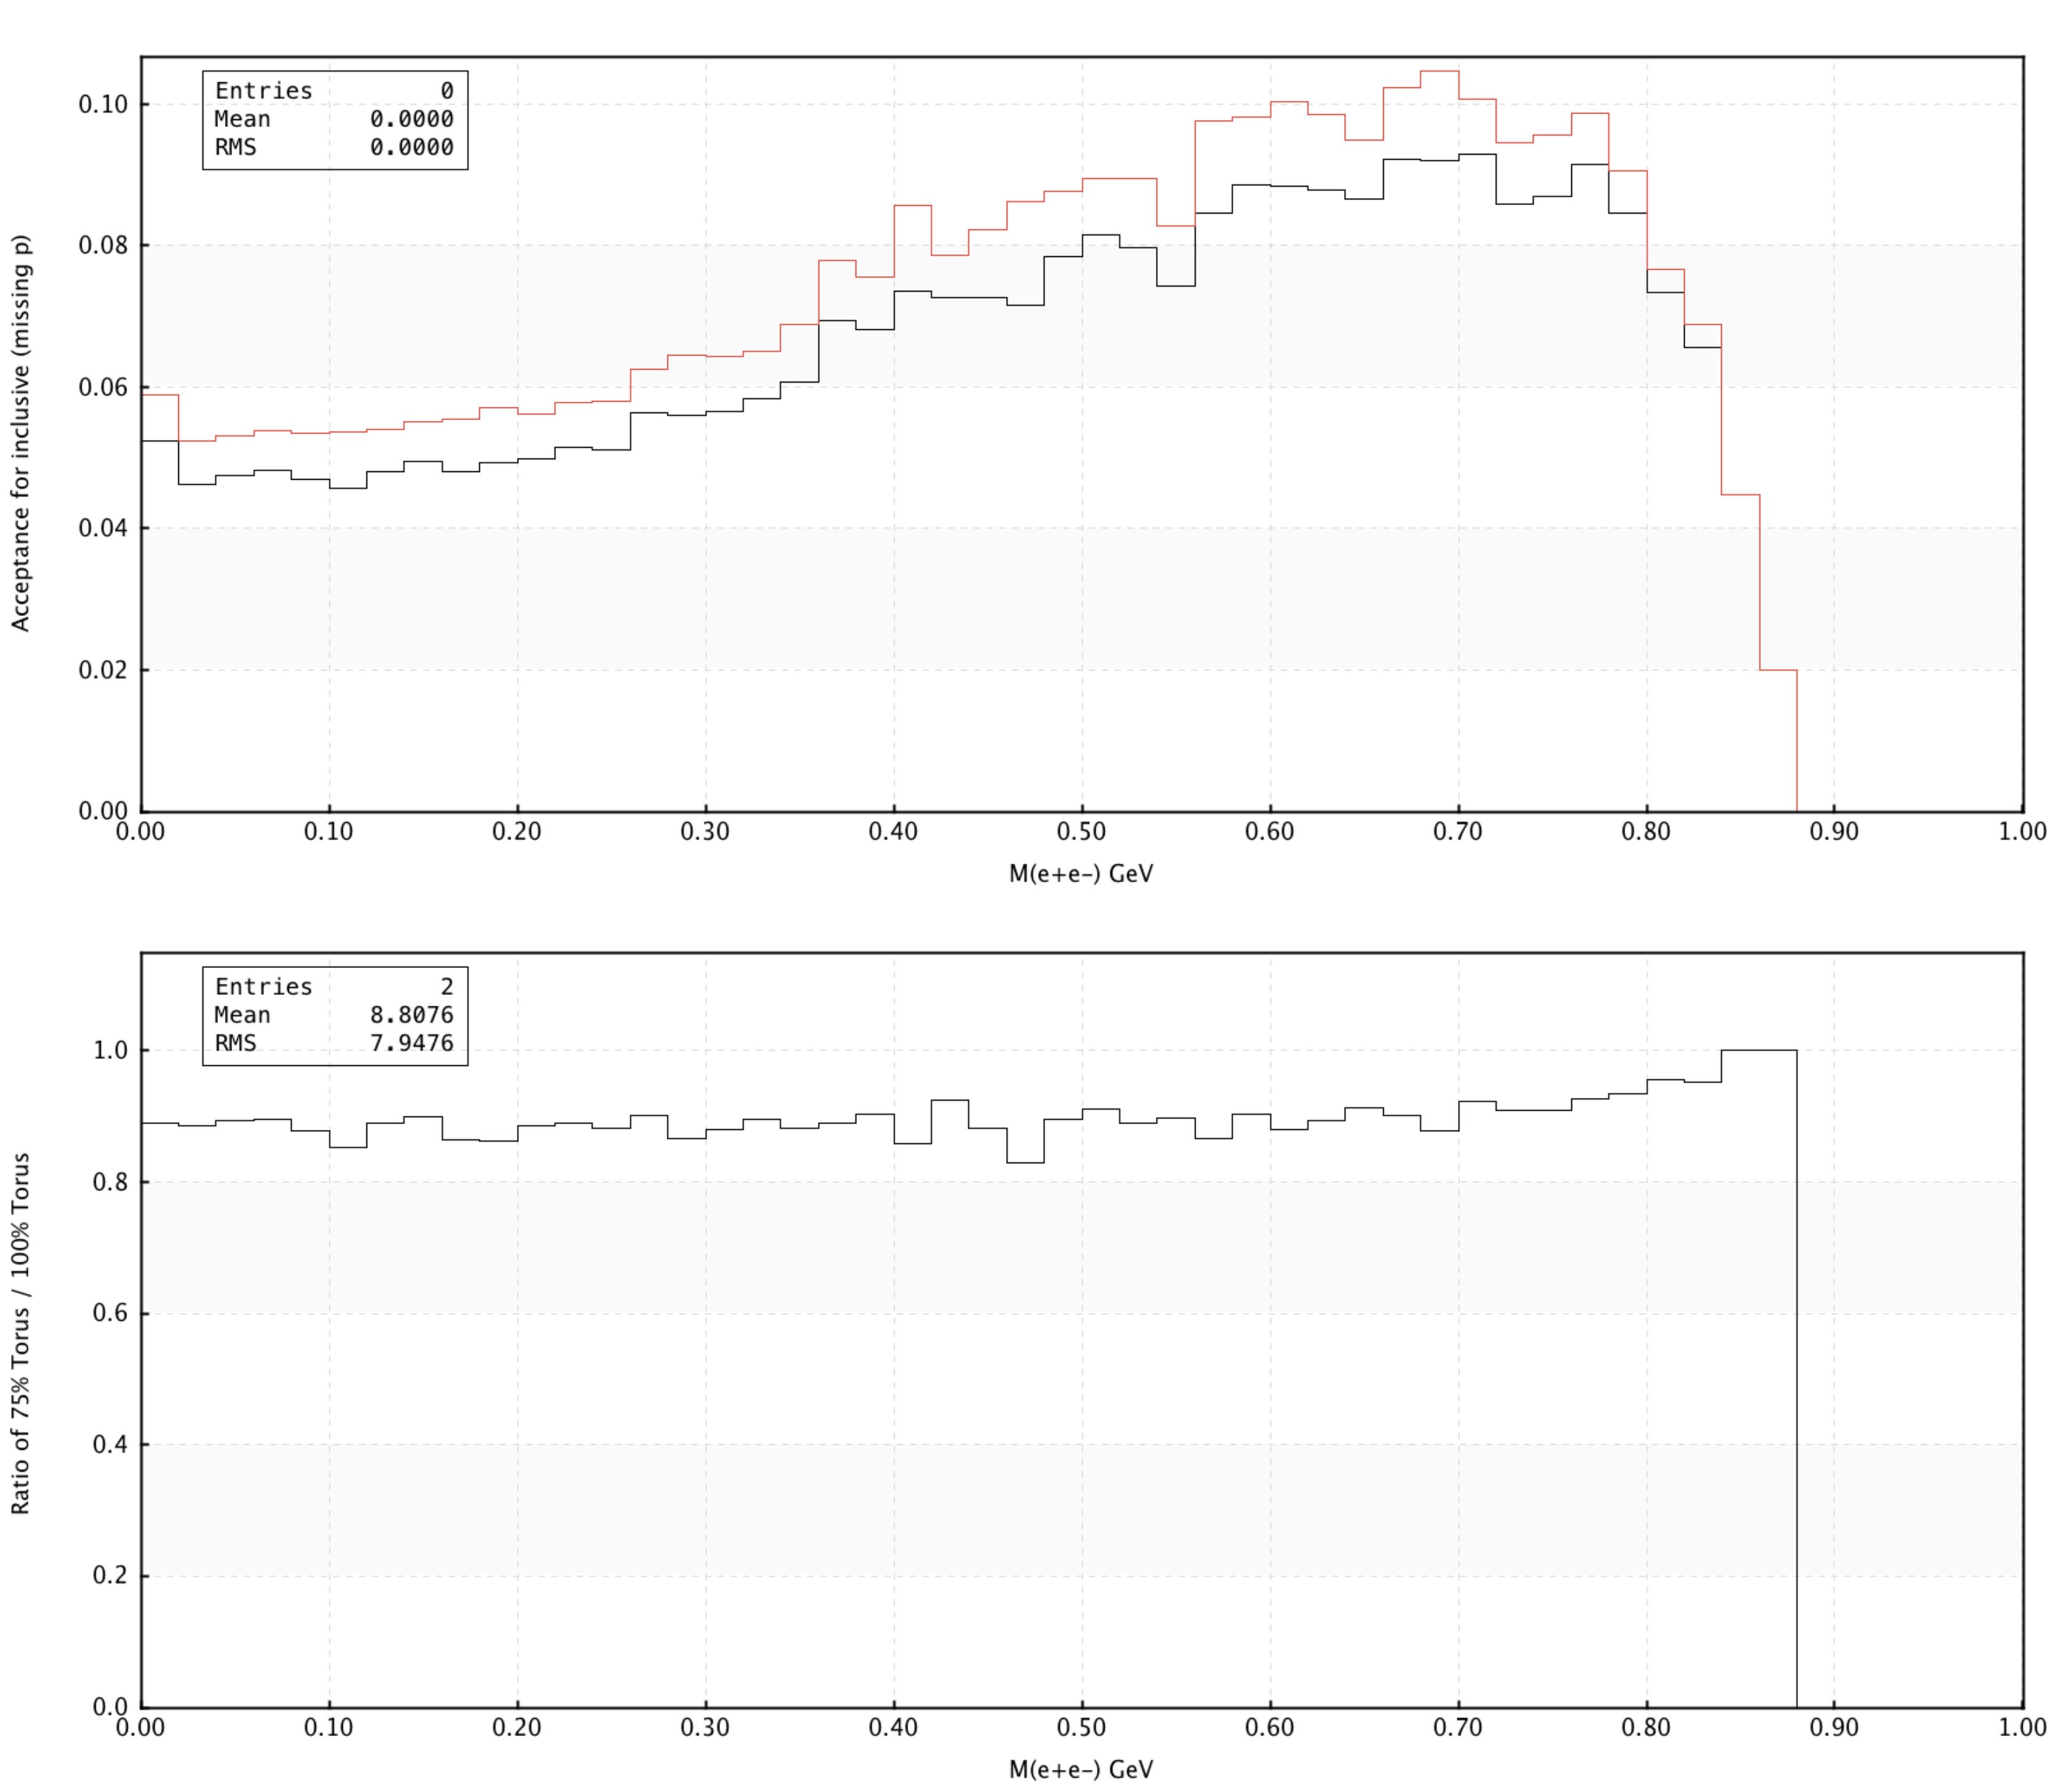
\includegraphics[width=\figwidth,height=1.6\qfigheight]{\grpath/counts/Ratio.pdf}
 		\caption[Acceptance, as a function of $M(\epem)$]{\label{fig:ratio}{Acceptance using a VMD decay model, as a function of $M(\epem)$ for the inclusive scheme(Top). The torus field was set to 75\%(red) as well as 100\%(black). Ratio of the acceptances plotted above (75\%/100\%)(Bottom). }}
\end{center}\end{figure}